\section{Structural Design}

The robotic leg is conceived as a three degrees of freedom (3-DOF) manipulator, a common simplification
of an insect's limb, designed to provide sufficient motion versatility within a robust and manageable structure.
The kinematic chain consists of three rigid links — Coxa, Femur, and Tibia — connected sequentially by three
revolute joints (from the robot's body toward the end-effector, as shown in Figure \ref{fig:hexapod_leg}):

\begin{itemize}
    \item \textbf{Hip Joint} ($q_1$): Connects the robot's body to the Coxa link and primarily controls the
        \textbf{yaw} motion of the leg, responsible for the lateral sweep relative to the body's longitudinal axis.
    \item \textbf{Knee Joint} ($q_2$): Connects the Coxa link to the Femur link and controls the
        \textbf{primary pitch} motion, enabling the lifting and lowering of the leg structure.
    \item \textbf{Ankle Joint} ($q_3$): Connects the Femur link to the Tibia link and controls the
        \textbf{secondary pitch} motion, significantly influencing the height and reach of the Foot (end-effector).
\end{itemize}

This configuration, is widely adopted in hexapod designs as it provides an optimal balance between complexity
and dexterity, allowing for effective gait planning and stable locomotion on various surfaces.

\begin{figure}[htbp]
    \centering
    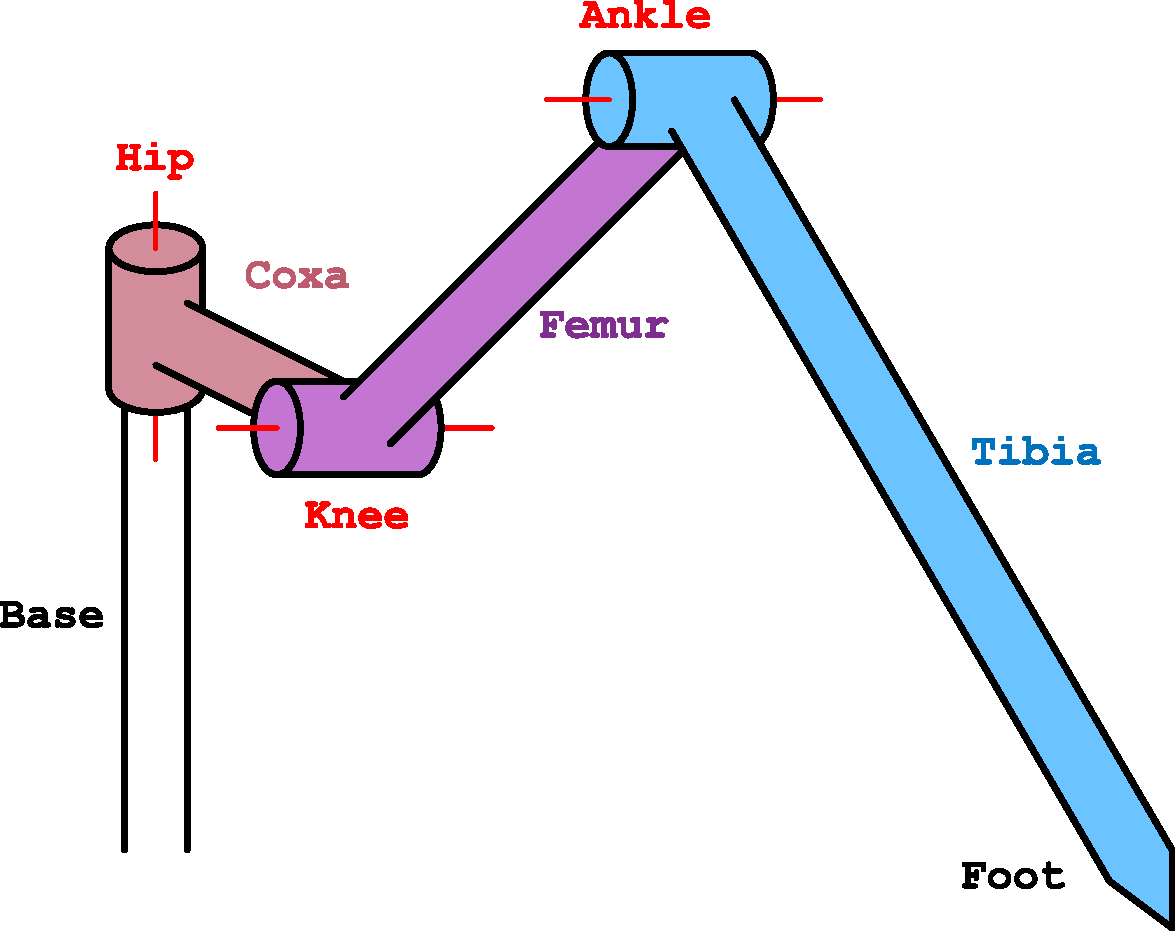
\includegraphics[width=0.8\textwidth]{images/hexapod-leg.pdf}
    \caption{Schematic Representation of the Mechanical Limb}
    \label{fig:hexapod_leg}
\end{figure}


\subsection{Limb Parametrization and Forward Kinematics}
\label{sec:dh_params}

The Denavit--Hartenberg (DH) convention \cite{denavit1955kinematic, siciliano2009robotics} is the standard
mathematical tool for describing the spatial relationships and defining the minimal parameter set required for
kinematic analysis of serial manipulators. By rigidly attaching coordinate frames to each link, DH enables a
standardized description of the link geometry and joint configuration.

The assignment of these frames follows a systematic methodology designed to isolate the four key parameters.
For a kinematic chain starting from a base frame $\{0\}$, a coordinate frame $\{i\}$ is rigidly attached to
link $i$. The most important rule is that the $z_i$-axis is placed along the axis of actuation (either
rotation or translation) for joint $i$. The $x_i$-axis is then constructed along the common normal connecting
$z_{i-1}$ (the previous joint axis) to $z_i$ (the current joint axis), with the origin of frame $\{i\}$
located at the intersection of $x_i$ and $z_i$. Finally, the $y_i$ axis is simply set to complete a
right-handed coordinate system.

Using this precise, rule-based placement of axes the entire transformation from frame $\{i\}$ to frame $\{i+1\}$
can now be described by a sequence of four fundamental operations tied directly to this geometry: the Link Length
($a_i$), Link Twist ($\alpha_i$), Link Offset ($d_i$), and the Joint Angle ($\theta_i$) (see Figure
\ref{fig:denavit_hartenberg}).

\begin{figure}[htbp]
    \centering
    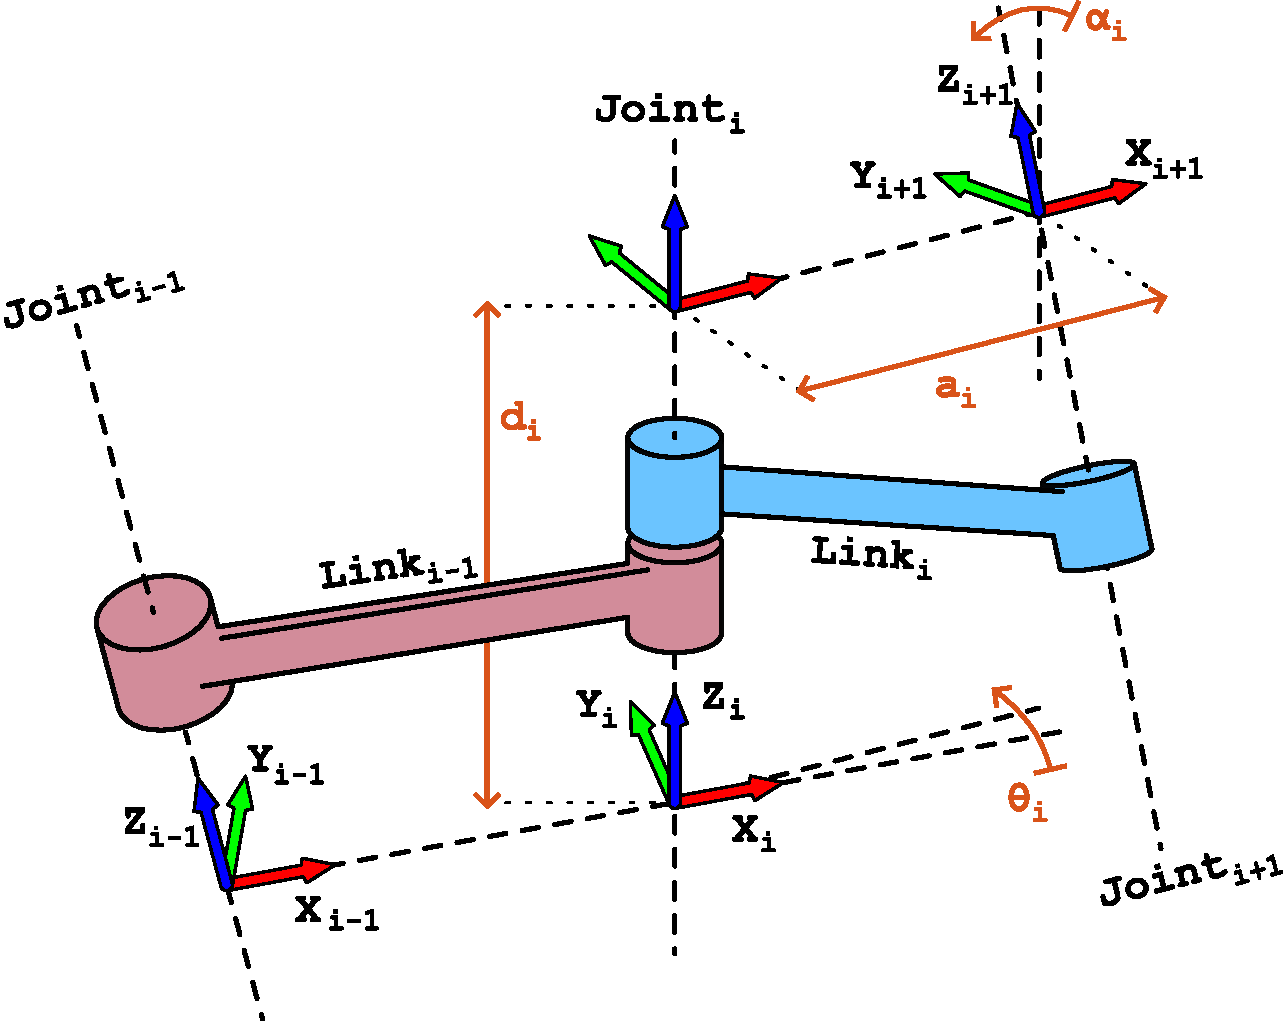
\includegraphics[width=0.8\textwidth]{images/denavit-hartenberg.pdf}
    \caption{Illustration of Denavit--Hartenberg Convention Parameters}
    \label{fig:denavit_hartenberg}
\end{figure}

The homogeneous transformation matrix, $T_{i}^{i+1}$, from frame $\{i\}$ to frame $\{i+1\}$, is given by:

\begin{equation}
    T_{i}^{i+1} = R_x(\alpha_i) \cdot T_x(a_i) \cdot R_z(\theta_i) \cdot T_z(d_i) =
    \begin{bmatrix}
        c_{\theta} & -s_{\theta} & 0 & a \\
        s_{\theta} c_{\alpha} & c_{\theta} c_{\alpha} & -s_{\alpha} & -ds_{\alpha} \\
        s_{\theta} s_{\alpha} & c_{\theta} s_{\alpha} & c_{\alpha} & dc_{\alpha} \\
        0 & 0 & 0 & 1
    \end{bmatrix}
\end{equation}

where the contracted notation $c_x = \cos(x), s_x = \sin(x)$ was used, while the overall transformation from
the base frame $\{b\}$ to the end-effector frame $\{e\}$, $T_b^e$, which is the Forward Kinematics solution,
is computed by the serial multiplication of these individual matrices:

\begin{equation}
    T_b^e = T_b^1 T_1^2 \dots T_{n-1}^n T_n^e
    \label{eqn:transf_matrix}
\end{equation}

To formally derive the Forward Kinematic model of the 3-DOF robotic limb, we apply the DH convention, following
the methodology introduced in the previous section. The assignment of the reference frames is shown in Figure
\ref{fig:assign_dh}, where the $z$-axes are represented in blue, $x$-axes in red and the $y$-axes are omitted.

Frame $\{b\}$ serves as the fixed base frame. In the context of a complete mobile hexapod, this frame is
typically attached to the center of the robot's main body to facilitate gait planning relative to the body's
center of gravity. However, for the experimental verification of the single modular limb in a benchtop setup,
frame $\{b\}$ is rigidly attached to the stationary mounting base, establishing a fixed reference for all
subsequent transformations.

\begin{figure}[htbp]
    \centering
    \begin{subfigure}[c]{0.48\textwidth}
        \centering
        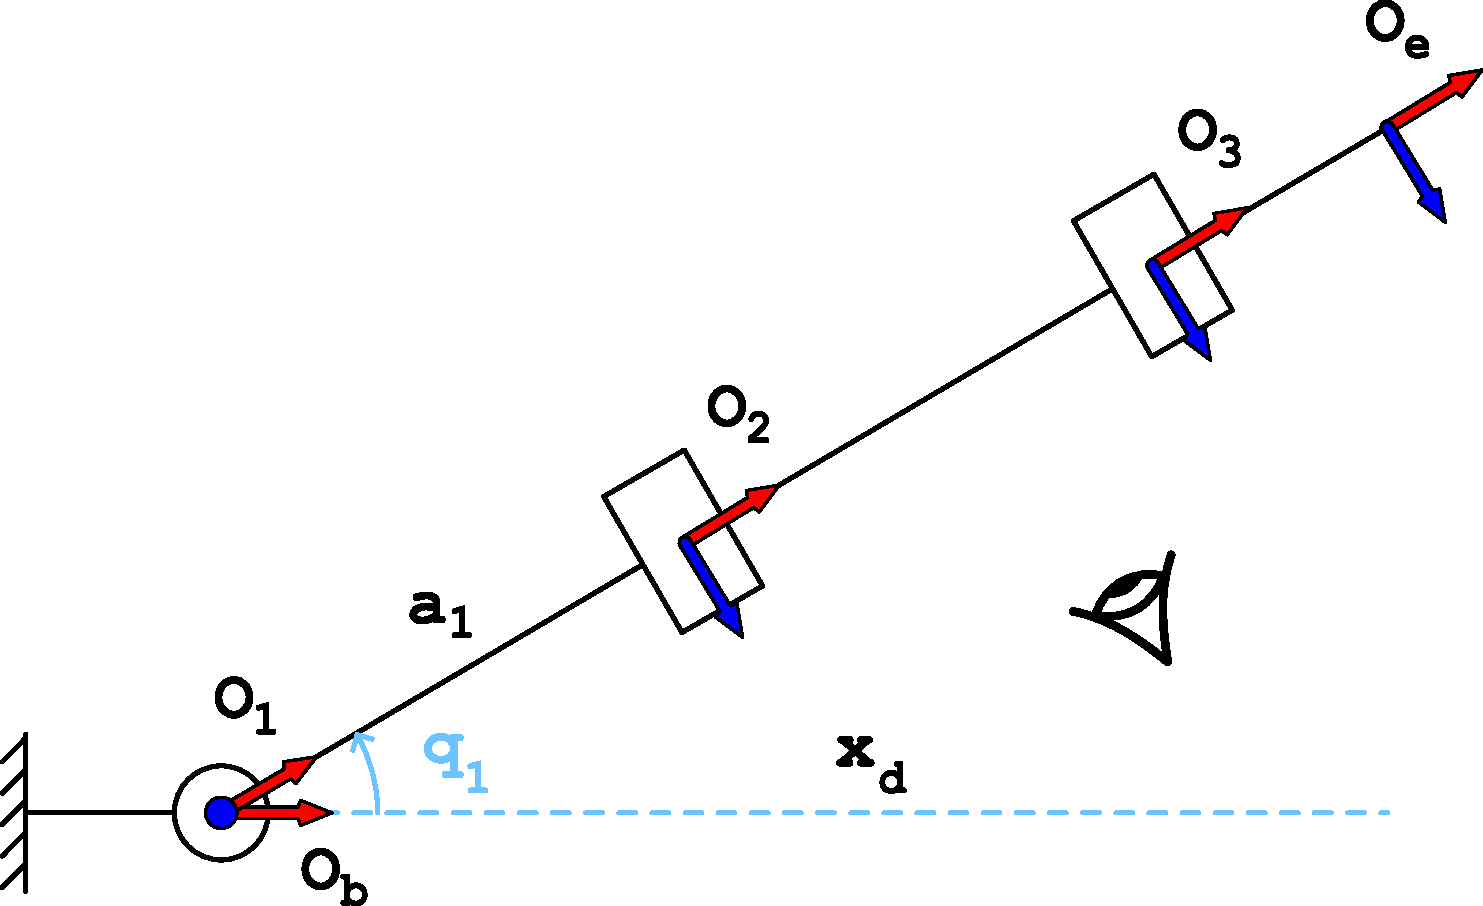
\includegraphics[width=\textwidth]{images/leg-top-dh.pdf}
        \caption{Top View}
        \label{fig:dh_top}
    \end{subfigure}
    \hfill
    \begin{subfigure}[c]{0.48\textwidth}
        \centering
        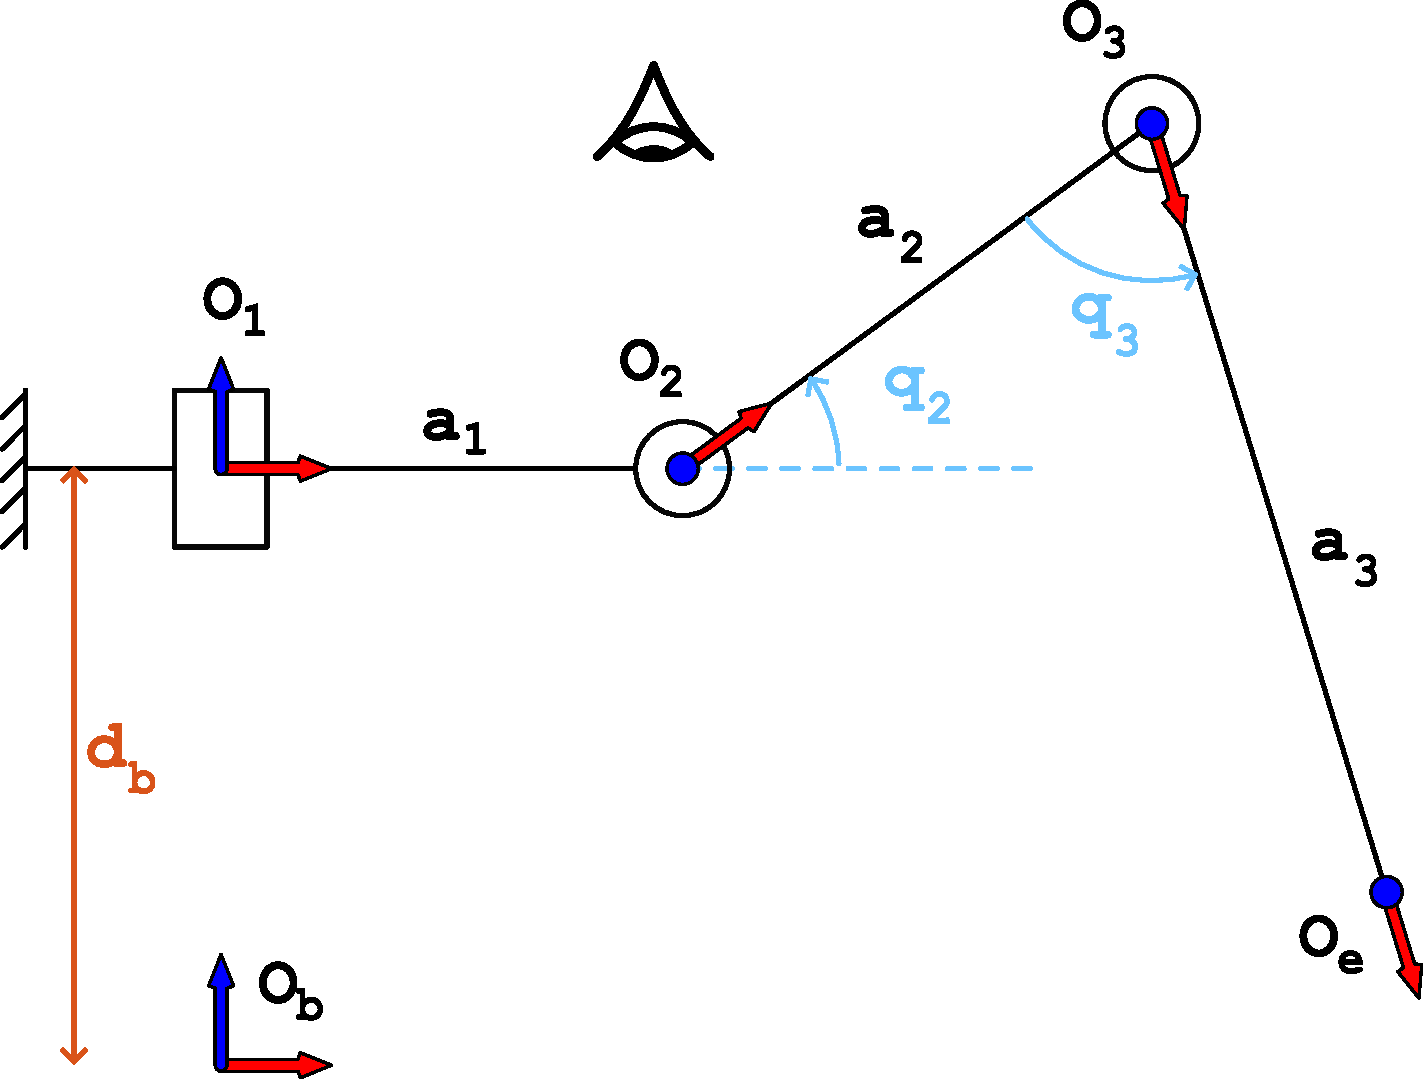
\includegraphics[width=\textwidth]{images/leg-side-dh.pdf}
        \caption{Side View}
        \label{fig:dh_side}
    \end{subfigure}
    \caption{Reference Frames and DH Parameters}
    \label{fig:assign_dh}
\end{figure}

Note the following key design choices:

\begin{itemize}
    \item The base offset $d_b$ represents the distance from the base frame $\{b\}$ to the frame of the Hip Joint
        (i.e. the mounting height of the leg on the base).
    \item The link lengths $a_1$, $a_2$ and $a_3$ correspond to the length of the Coxa, Femur and Tibia links,
        respectively. These values are chosen based on a mix of aesthetics and physical constraints. More
        specifically, the Coxa length is minimized and the Femur length is chosen to be smaller than the Tibia
        length.
    \item The twist angle $\alpha_1 = 90^{\circ}$ is necessary because the axis of the Knee Joint ($z_2$) is
        orthogonal to the axis of the Hip Joint ($z_1$).
    \item Subsequent frames are coplanar, resulting in zero twist angles ($\alpha_2 = \alpha_3 = 0^{\circ}$)
        and link offsets ($d_1 = d_2 = d_3 = 0\ mm$), simplifying the transformation matrices.
    \item The joint angle $q_3$ is rotated by an extra $-180^\circ$ to simplify IK derivation and match the
        hardware implementation.
    \item Since the attitude of the end-effector is irrelevant, the final joint angle for the Tibia link is
        fixed at $\theta_4 = 0$, as the end-effector (Foot) frame $\{e\}$ is placed at the tip of the Tibia
        link, defining the final link length $a_3$.
\end{itemize}

The parameter for the DH model are reported in Table \ref{tab:dh_parameters}.

\begin{table}[htbp]
    \centering
    \begin{tabular}{c c c c c}
        \hline
        \textbf{Link} & \textbf{$a$ [mm]} & \textbf{$\alpha$ [deg]} & \textbf{$d$ [mm]} & \textbf{$\theta$ [deg]} \\
        \hline
        \hline
        Base    & $0$           & $0$   & $d_b = 178$   & $q_1$         \\
        Coxa    & $a_1 = 40$    & $90$  & $0$           & $q_2$         \\
        Femur   & $a_2 = 78$    & $0$   & $0$           & $q_3 - 180$   \\
        Tibia   & $a_3 = 132$   & $0$   & $0$           & $0$           \\
        \hline
    \end{tabular}
    \caption{Denavit--Hartenberg Parameters of the Limb}
    \label{tab:dh_parameters}
\end{table}


\subsection{Inverse Kinematics Overview and Derivation}

Forward Kinematics analysis allows for the straightforward computation of the end-effector's pose starting from a
known joint configuration. However, this direct mapping is often impractical for high-level control. Defining a
task or a trajectory is inherently more intuitive in Cartesian space (e.g. coordinates in the world frame) than
in the abstract joint space. Consequently, to command the robot to reach a specific physical location, the
inverse problem must be addressed.

Inverse Kinematics (IK) \cite{siciliano2009robotics} is the problem of determining the set of joint variables,
$q = [q_1, \dots, q_n]$, required to place the end-effector at a desired pose, $p_d = [x_d, y_d, z_d, \phi_d, \theta_d, \psi_d]^T$.
Unlike Forward Kinematics, the IK problem is fundamentally more challenging due to the non-linear relationship
between joint space and Cartesian space. The mathematical objective is to solve the inverse mapping:
\begin{equation*}
    q = f^{-1}(p_d)
\end{equation*}

The complexity of the problem stems from several factors. Solutions may be non-unique, meaning multiple
joint configurations can achieve the same end-effector pose and/or non-existent if the target pose lies outside
the robot's physical workspace. Furthermore, singularities — joint configurations that cause a loss of effective
degrees of freedom — must be avoided as they lead to control instability.

To address these challenges, solution approaches usually fall into two main categories: on one side, analytical
solutions provide closed-form, explicit equations for the joint variables as a function of the desired pose,
offering high computational efficiency and usually providing all possible solutions. They are generally preferred
for manipulators with simple geometries. Numerical Methods, conversely, use iterative algorithms to converge on a
solution by minimizing a position error function. While they are necessary for complex kinematic structures
lacking analytical solutions, they are less computationally efficient and provide only one solution per iteration.

Given the simple structure of the application, an analytical solution can be found using planar geometry and
fundamental trigonometric relationships. For the derivation, the leg geometry is conceptually separated into two
different point of views, to facilitate the calculation. Figure \ref{fig:find_ik} depicts a schematic representation
of them.

\begin{figure}[htbp]
    \centering
    \begin{subfigure}[t]{0.48\textwidth}
        \centering
        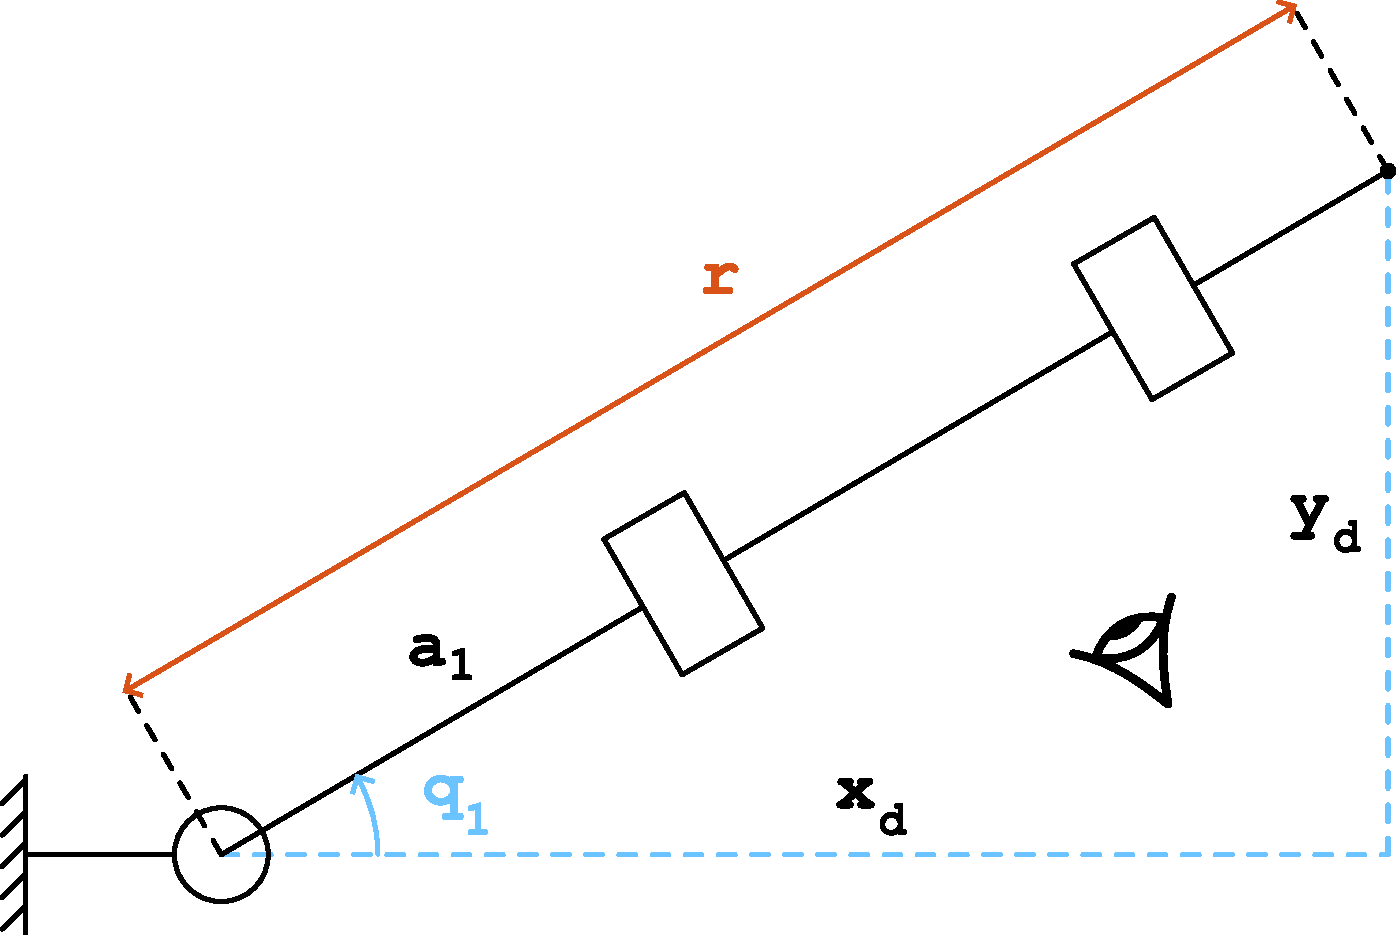
\includegraphics[width=\textwidth]{images/leg-top-ik.pdf}
        \caption{Top View}
        \label{fig:ik_top}
    \end{subfigure}
    \hfill
    \begin{subfigure}[t]{0.48\textwidth}
        \centering
        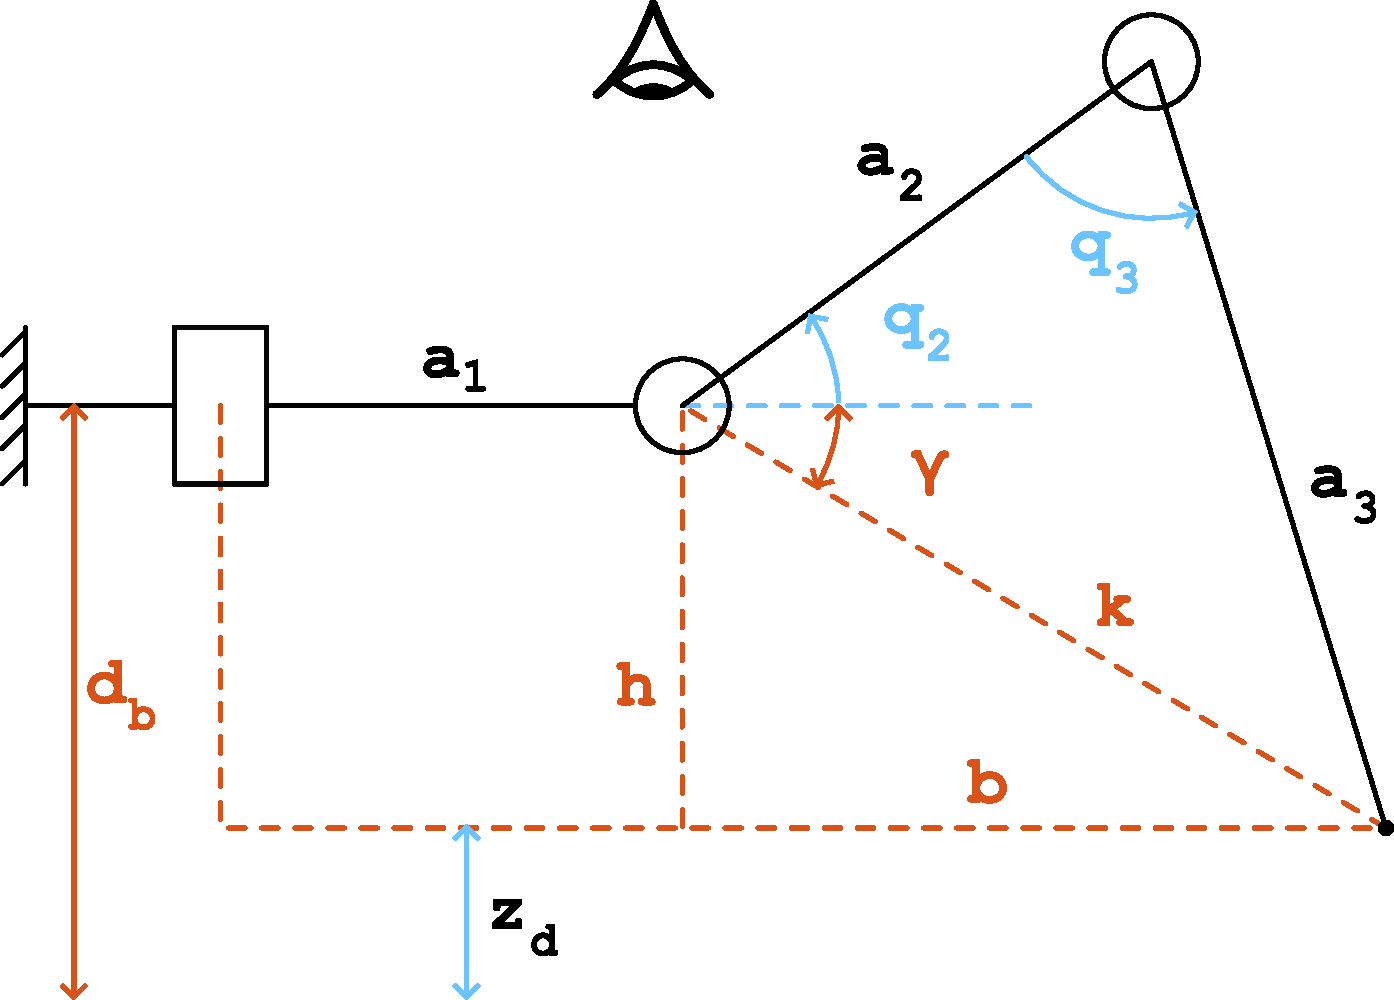
\includegraphics[width=\textwidth]{images/leg-side-ik.pdf}
        \caption{Side View}
        \label{fig:ik_side}
    \end{subfigure}
    \caption{Leg Geometry for IK Derivation}
    \label{fig:find_ik}
\end{figure}

Given a desired end-effector position $p_d = [x_d, y_d, z_d]^T$, the three required joint angles $q_1, q_2, q_3$
can be determined sequentially as follows:


\subsubsection{Joint Angle $q_1$ (Yaw)}

The first joint angle, $q_1$, is determined solely by the $X$ and $Y$ coordinates of the desired position,
representing a rotation in the horizontal plane (Figure \ref{fig:ik_top}). This is a straightforward calculation:
\begin{equation*}
    q_1 = \operatorname{atan2}(y_d,x_d)
\end{equation*}
The $\operatorname{atan2}$ function ensures that the resulting angle correctly accounts for the sign of the
coordinates across all four quadrants, providing the correct angle $\theta \in [-\pi, \pi]$.


\subsubsection{Joint Angles $q_2$ and $q_3$ (Pitch)}

The derivation of $q_2$ and $q_3$ is performed in the vertical plane (Figure \ref{fig:ik_side}),
which is defined by the Femur and Tibia links. We first define a set of auxiliary geometric variables:
\begin{itemize}
    \item \textbf{Projected Radial Distance ($r$):} The distance from the origin to the end-effector projected
        onto the $XY$-plane.
        \begin{equation*}
            r = \sqrt{x_d^2 + y_d^2}
        \end{equation*}
    \item \textbf{Horizontal Distance ($b$):} The effective horizontal distance from the $q_2$ joint axis to
        the end-effector.
        \begin{equation*}
            b = r - a_1 \Leftarrow r = b + a_1
        \end{equation*}
    \item \textbf{Vertical Distance ($h$):} The effective vertical distance from the $q_2$ joint axis to
        the end-effector.
        \begin{equation*}
            h = d_b - z_d
        \end{equation*}
    \item \textbf{Virtual Link Length ($k$):} The length of the virtual link connecting the $q_2$ joint axis
        to the end-effector, forming the third side of the triangle with links $a_2$ and $a_3$.
        \begin{equation*}
            k = \sqrt{h^2 + b^2}
        \end{equation*}
    \item \textbf{Knee Offset Angle ($\gamma)$:} The angle between the continuation of $a_1$ and the
        virtual link length $k$.
        \begin{equation*}
            \gamma = \operatorname{atan2}(h, b)
        \end{equation*}
        Using $\operatorname{atan2}$ ensures once again correctness even when $h$ is negative, i.e. when the
        Foot is above the body of the robot.
\end{itemize}

Using these auxiliary variables, the final joint angles $q_2$ and $q_3$ can now be obtained.

The second joint angle, $q_2$, is found by determining the internal angle of the $a_2, a_3, k$ triangle
using the Law of Cosines and compensating for the angle ($\gamma$):
\begin{equation*}
    q_2 = \operatorname{acos}\left(\frac{a_2^2 + k^2 - a_3^2}{2 \cdot a_2 \cdot k}\right) - \gamma
\end{equation*}
The third and final joint angle, $q_3$, is the angle between the $a_2$ and $a_3$ links. This is again derived
from the Law of Cosines:
\begin{equation*}
    q_3 = \operatorname{acos}\left(\frac{a_2^2 + a_3^2 - k^2}{2 \cdot a_2 \cdot a_3}\right)
\end{equation*}

Substituting the intermediate variables back into the expressions for $q_2$ and $q_3$ yields the final,
consolidated IK equations as a direct function of the desired end-effector coordinates as reported in Appendix
\ref{app:ik}.
